% !TEX root =  ../../master.tex
\section{Client}
\label{sec:ClientKonzept}

Wie bereits in Kap. \vref{ssec:React} beschrieben, wird in diesem Projekt React verwendet. 
Für die Unterteilung der verschiedenen Komponenten soll auf eine spezielle \acfp{UX} und \acfp{UI} wert gelegt werden. 
Da die Applikation im Rahmen eines Projektes der DHBW Mannheim konzeptioniert wird, sollen die Komponenten an dieses Farbschema angelehnt werden. 
Im folgenden soll auf den grundlegende Aufbau bzw. die grundlegende Idee der Benutzeroberfläche beim Start des Projektes eingegangen werden. 
Die gezeigten Mockups erheben dabei keinen Anspruch vollständig zu sein, da diese lediglich zur groben Orientierung und Ausrichtung benötigt werden.

% !TEX root =  ../../master.tex
\subsection{Grundgerüst}

Um auf den einzelnen Unterseiten der Anwendung einen Anhaltspunkt zu besitzen, ist die Abbildung \ref{fig:MockGrundgeruest} da. 
In dieser wird eine grundlegende Struktur festgelegt, welche auf den Unterseiten der Webanwendung verwendet werden soll.
Dabei wird die Seite in unterschiedliche Sektoren untergliedert.
Die einzelnen Komponenten einer Seite sind dabei der \emph{Header}, \emph{Inhalt der Seite}, sowie der \emph{Footer}. 
Wie schon die Namen der Sektoren indizieren, ist die Anordnung von \emph{Header} über den \emph{Inhalt der Seite} zu dem abschließenden \emph{Footer}, strukturiert.
Jedoch besitzen diese Komponenten nicht die maximale Breite.
Daher gibt es an den rechten und linken Rand der Seite jeweils ungenutzte Fläche. 
Diese freie Fläche ist jedoch gewollt, dadurch soll der Benutzer nicht mit zu viel Inhalt auf einmal konfrontiert werden.
Somit kann seine Aufmerksamkeit auf den \emph{Inhalt der Seite} gelenkt werden.
Als Vorteil besitzt ein konsistenter Aufbau, dass sich der Benutzer an eine Struktur gewöhnen kann. 

\begin{figure}[H]
	\centering
	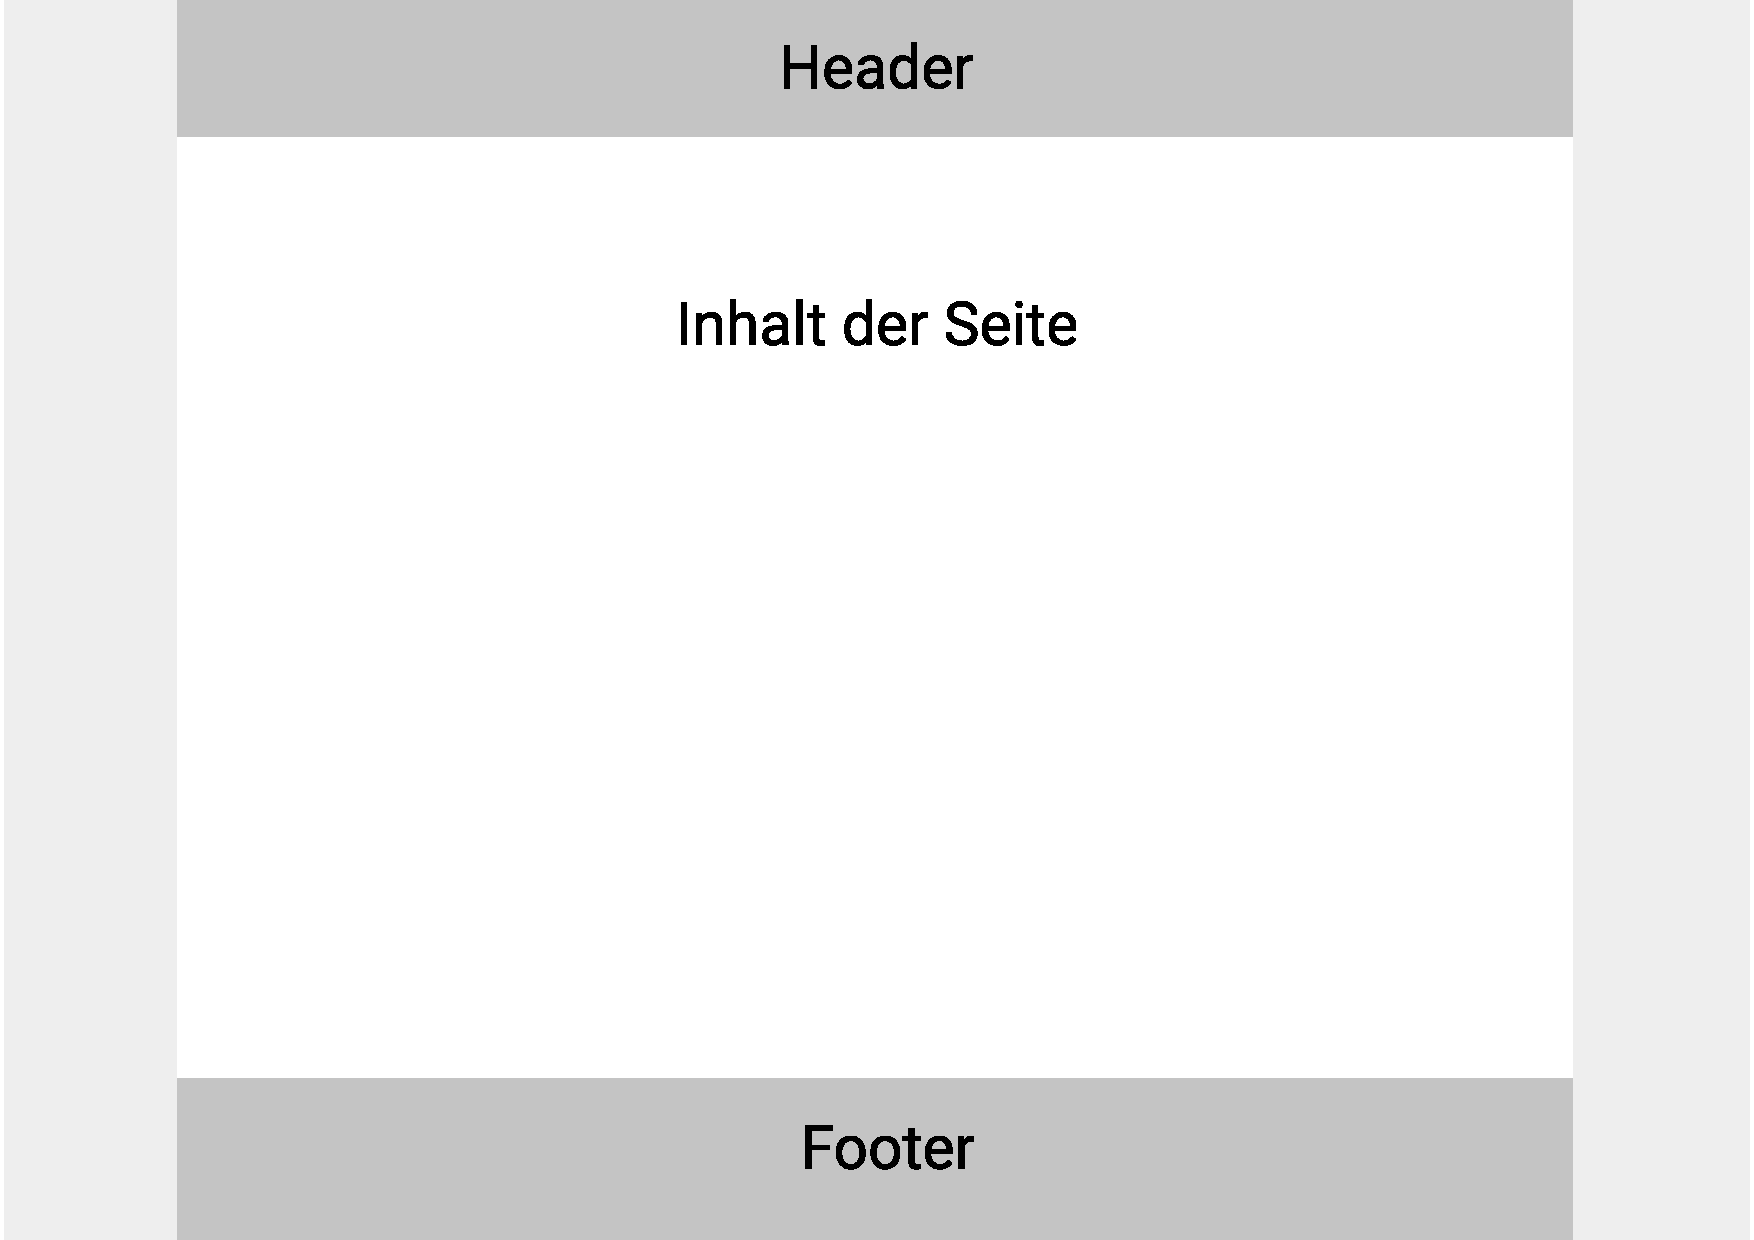
\includegraphics[width=0.7\textwidth]{img/konzeption/client/grundgeruest}
	\captionsetup{justification=centering, format=plain}
	\caption[Mock-Up vom Grundgerüst der Anwendung]{Mock-Up vom Grundgerüst der Anwendung \\\figma}
	\label{fig:MockGrundgeruest}
\end{figure}


\subsection{Teilnahme und Login}

Beim ersten Laden der Anwendung soll eine Startseite aufgebaut werden, wie sie in Abbildung~\vref{fig:MockSignin} zu sehen ist.
Hierbei sollen Nutzer einfach an einer Umfrage teilnehmen und sich anmelden oder ein Registrierungsvorgang starten können.
Für die Teilnahme an einer Umfrage müssen die Studierenden lediglich einen \emph{Surveycode} wie \zb \texttt{W3VFG5NHY} eingeben.
Eine Anmeldung ist nicht erforderlich, um die Anonymität gemäß Anforderung~\hyperref[Anf:A14]{A14} zu wahren.
Anschließend wird der Benutzer auf die Umfrageseite weitergeleitet, auf der er die benötigten Felder ausfüllt (siehe Kapitel~\ref{ssec:konzept:client:umfrage}).
Beim Beantworten von Umfragen ist davon auszugehen, dass dies zu einem großen Teil von mobilen Endgeräten erfolgt (siehe Anforderung~\hyperref[Anf:A1]{A1}).
Diese Seiten müssen daher für die mobile Nutzung optimiert werden, dies ist jedoch nicht als Teil der Mock-Ups dargestellt.
Für angemeldete Benutzer, die Umfragen erstellen und verwalten, ist jedoch die mobile Nutzung unwahrscheinlich, da etwa Dozenten in der Regel die Vorlesungsvorbereitung an einem Desktop-Computer durchführen.
% Hierbei soll der späteren Implementierung dieser Seite der Aspekt der mobilen Benutzung beachtet werden, da viele Benutzer eine Umfrage auf ihren mobilen Endgeräten durchführen.
% Bei allen anderen Seiten soll dieser Aspekt jedoch zunächst vernachlässigt werden.

\begin{figure}[H]
	\centering
	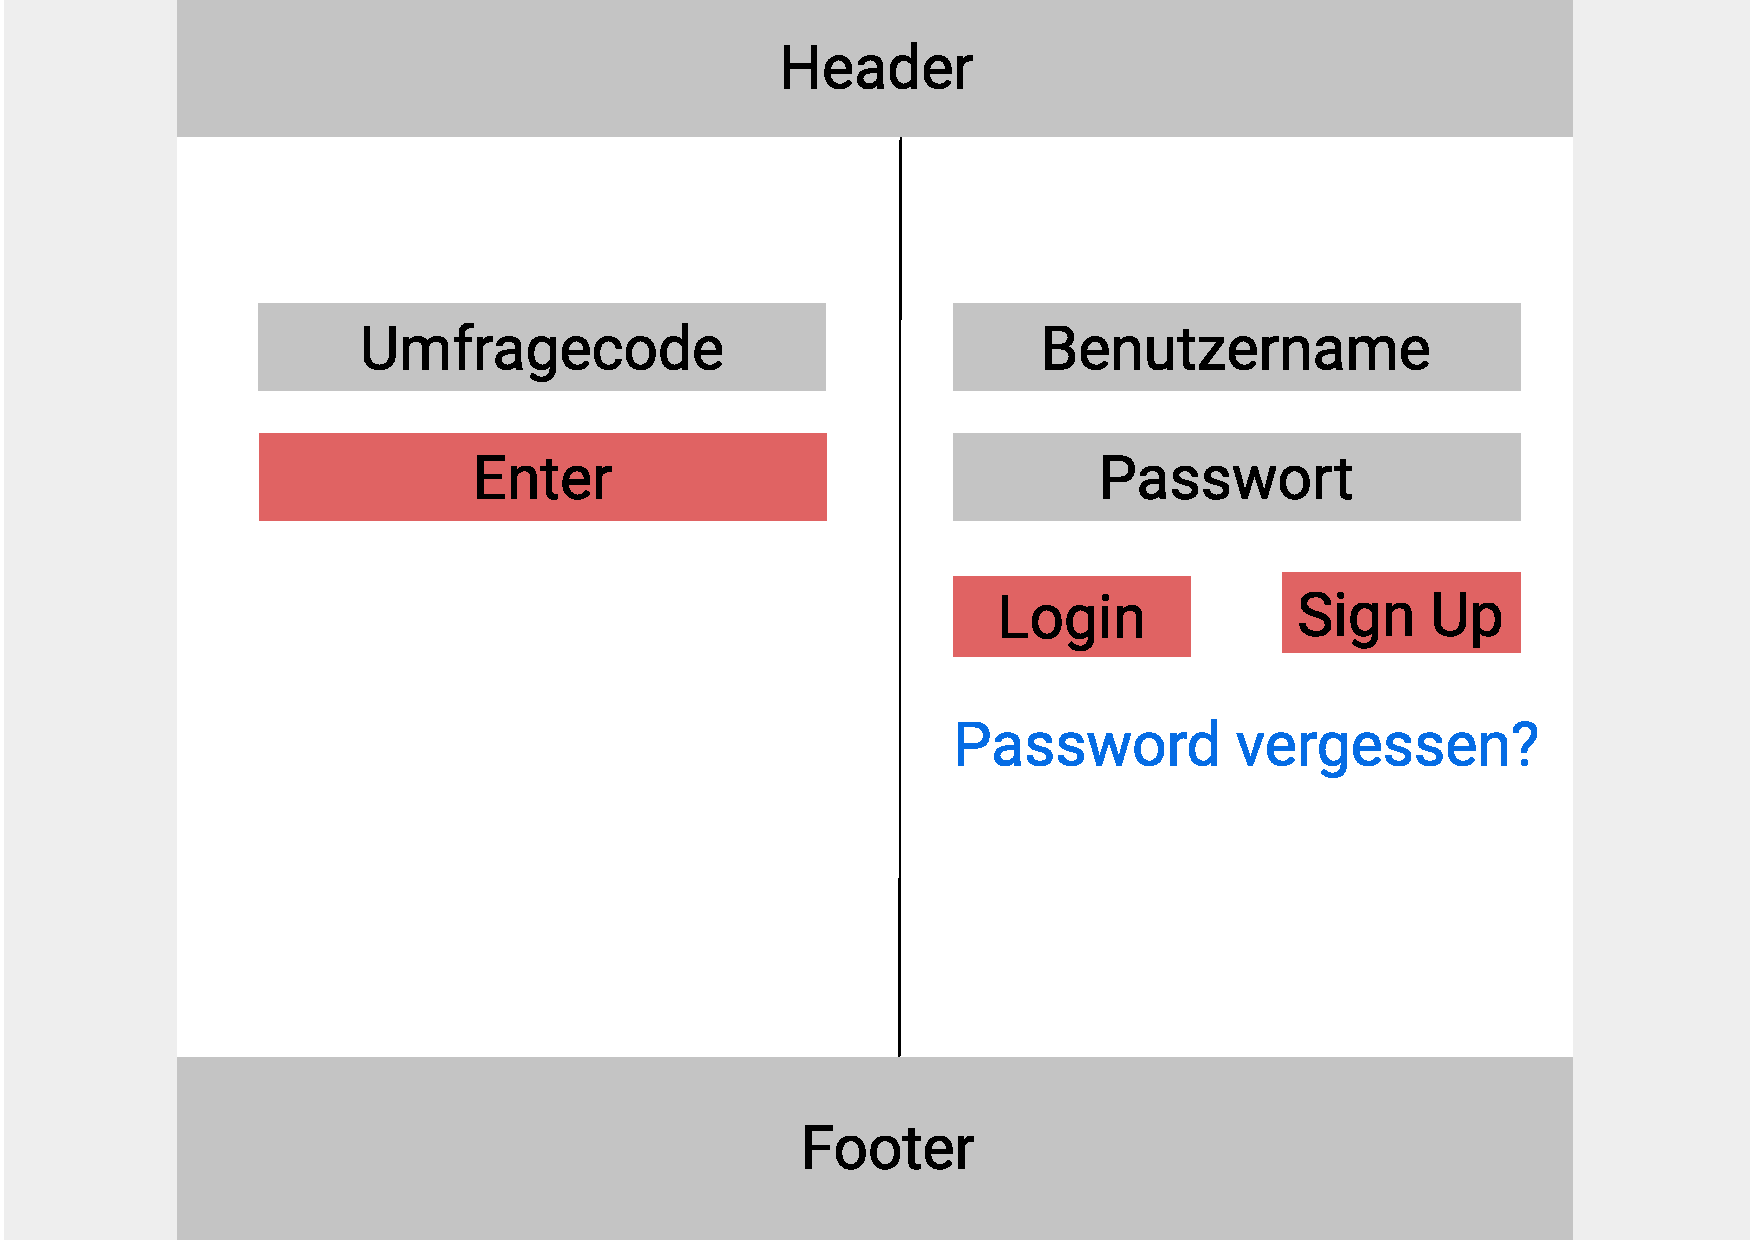
\includegraphics[width=0.7\textwidth]{img/konzeption/client/signin}
	\captionsetup{justification=centering, format=plain}
	\caption[Mock-Up der Startseite]{Mock-Up der Startseite \\\figma}
	\label{fig:MockSignin}
\end{figure}

Nutzer erhalten, wie in Abbildung~\ref{fig:MockSignin} auf der rechten Seiten sichtbar, ebenfalls die bereits angesprochene Anmelde-Möglichkeit.
Hierzu soll der \emph{Benutzername} und das \emph{Passwort} eines existierenden Benutzers eingegeben werden.
Nach einer erfolgreichen Anmeldung soll der Benutzer auf die Dashboard-Seite weitergeleitet werden (siehe Kapitel~\ref{ssec:konzept:client:dashboard}).
Bei der ersten Nutzung der Anwendung besteht die Möglichkeit über den Knopf \emph{Sign Up} ein Registrierungsvorgang gestartet werden, was zunächst eine Weiterleitung auf die Registrierungsseite (siehe Kapitel~\ref{ssec:konzept:client:dashboard}) vorsieht.
Dadurch wird Anforderung~\hyperref[Anf:A10]{A10}, die manuelle Veröffentlichung einer Umfrage, sowie Anforderung~\hyperref[Anf:A15]{A15}, die Möglichkeit zur einfachen Teilnahme an Umfragen, erfüllt.


\subsection{Signup}
\label{ssec:konzept:client:signup}
Um eine Umfrage erstellen zu können, an der Umfrageteilnehmer partizipieren können, muss zuvor ein Nutzerkonto erstellt werden. 
Hierfür wählt der Benutzer wie in Abb. \ref{fig:MockSignup} dargestellt das Formfeld mit seinem Benutzernamen wie \zb \emph{\texttt{Martin}}. 
Danach wird die E-Mail des Benutzers verlangt, um die Person verifizieren zu können. 
Inwiefern die Identifizierung von den Benutzern geschieht, ist zum Zeitpunkt der Erstellung der Mockups noch nicht klar. 
Eine Möglichkeit, worauf sich in diesem Mockup bezogen wird, ist jedoch die Authentifizierung über die E-Mail-Adresse der DHBW. 
Anschließend wählt der Benutzer ein Passwort seiner Wahl. 
Ist das gewählte Passwort konkludent, so wird der Benutzer angelegt.
Durch das wiederholte eingeben des Passwortes wird sichergestellt, dass es zu keiner Verwirrung bezüglich des gesetzten Passwortes kommt. 
Mit der wiederholten Eingabe des Kennwortes, wird der Nutzer bei unkonkludenten Passwörtern mit einer Fehlermeldung darauf hingewiesen.

\begin{figure}[H]
	\centering
	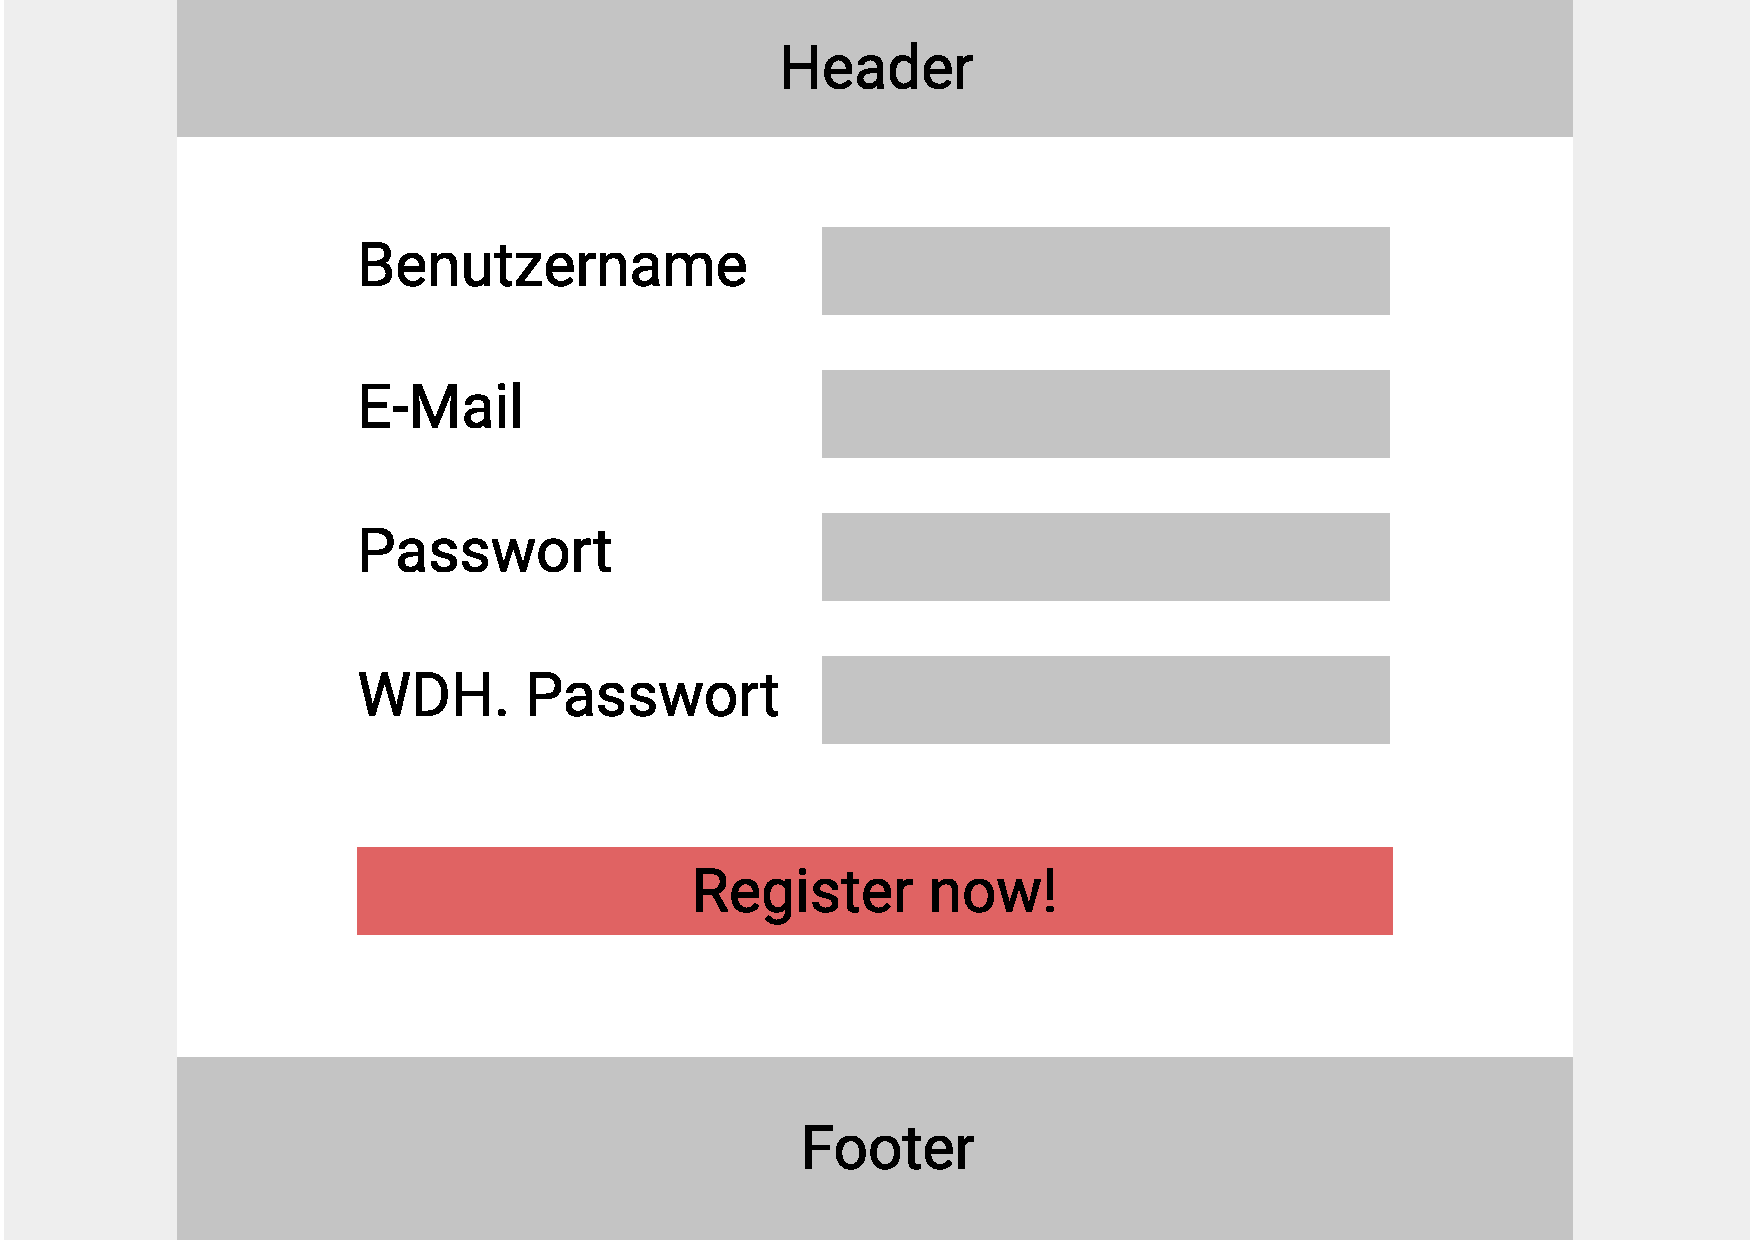
\includegraphics[width=0.7\textwidth]{img/konzeption/client/register}
	\captionsetup{justification=centering, format=plain}
	\caption[Mock-Up der Startseite]{Mock-Up der Registierungsseite \\\figma}
	\label{fig:MockRegister}
\end{figure}

\subsection{Umfrage}
\label{ssec:konzept:client:umfrage}
Wie in Abbildung~\vref{fig:MockUmfrageTeilnehmer} dargestellt, wird der Teilnehmer auf die zuvor angegebene Umfrage geleitet.
Die Fragen werden dabei jeweils in einer eigenen Karte dargestellt.
Durch Drücken eines Knopfes soll der Teilnehmer zur nächsten Frage gelangen.
Gleichzeitig soll dem Benutzer sein Fortschritt verdeutlicht werden, um die Dauer der Umfrage abschätzen zu können.
Die Abgabe der Umfrage erfolgt identisch zum Fragenwechsel.
Der Teilnehmer soll dabei Feedback erhalten, ob seine Teilnahme erfolgreich war.

Durch diesen Vorgang sollen die Anforderungen~\hyperref[Anf:A14]{A14}, die anonyme Teilnahme, sowie \hyperref[Anf:15]{A15}, die einfache Teilnahme an einer Umfrage, erfüllt werden.

\begin{figure}[H]
	\centering
	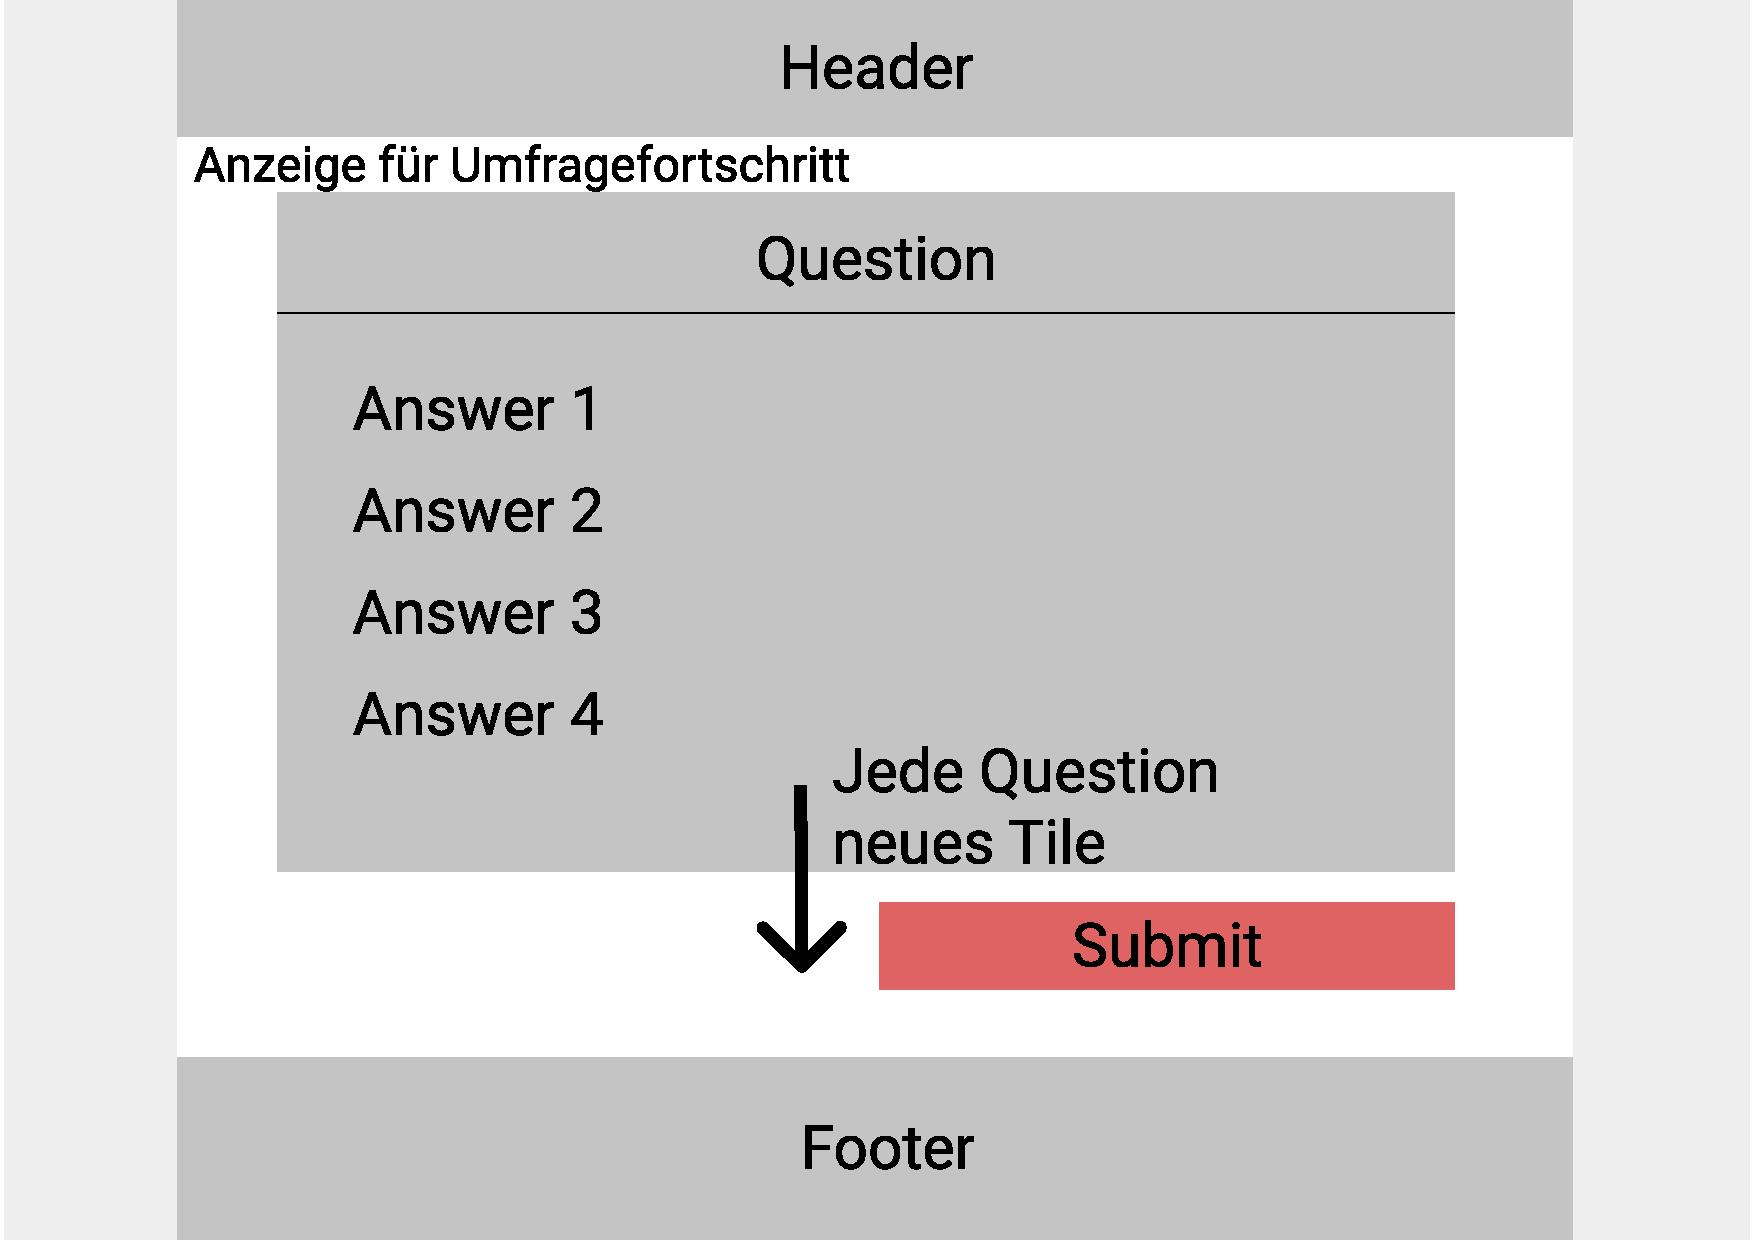
\includegraphics[width=0.7\textwidth]{img/konzeption/client/umfrage_teilnehmer}
	\captionsetup{justification=centering, format=plain}
	\caption[Mock-Up der Teilnahmeseite]{Mock-Up der Teilnahmeseite\\\figma}
	\label{fig:MockUmfrageTeilnehmer}
\end{figure}


\subsection{Result-Dashboard}
\label{ssec:konzept:client:dashboard}

Das Dashboard soll die Kernkomponente dieser Anwendung sein. 
Auf dieser sollen sämtliche Umfragen und deren Ergebnisse dargestellt werden, wie es in Abbildung \ref{MockDashboard} zu sehen ist.
Über eine klickbare Auflistung, welche auf der linken Seite der Abbildung zu sehen ist, soll eine Navigation über die Umfragen erfolgen.
Beim Anklicken einer Umfrage sollen die Diagramme und Auswertungen entsprechend geladen und angezeigt werden, sodass der Nutzer die Resulate der Umfrage überblicken kann.
Dabei soll pro Frage ein Diagramm erstellt werden, dessen Typ sich an der Frageart orientiert.
Beispielsweise wird bei einer Single-Choice-Frage ein Kreisdiagramm erstellt.

\begin{figure}[h]
	\centering
	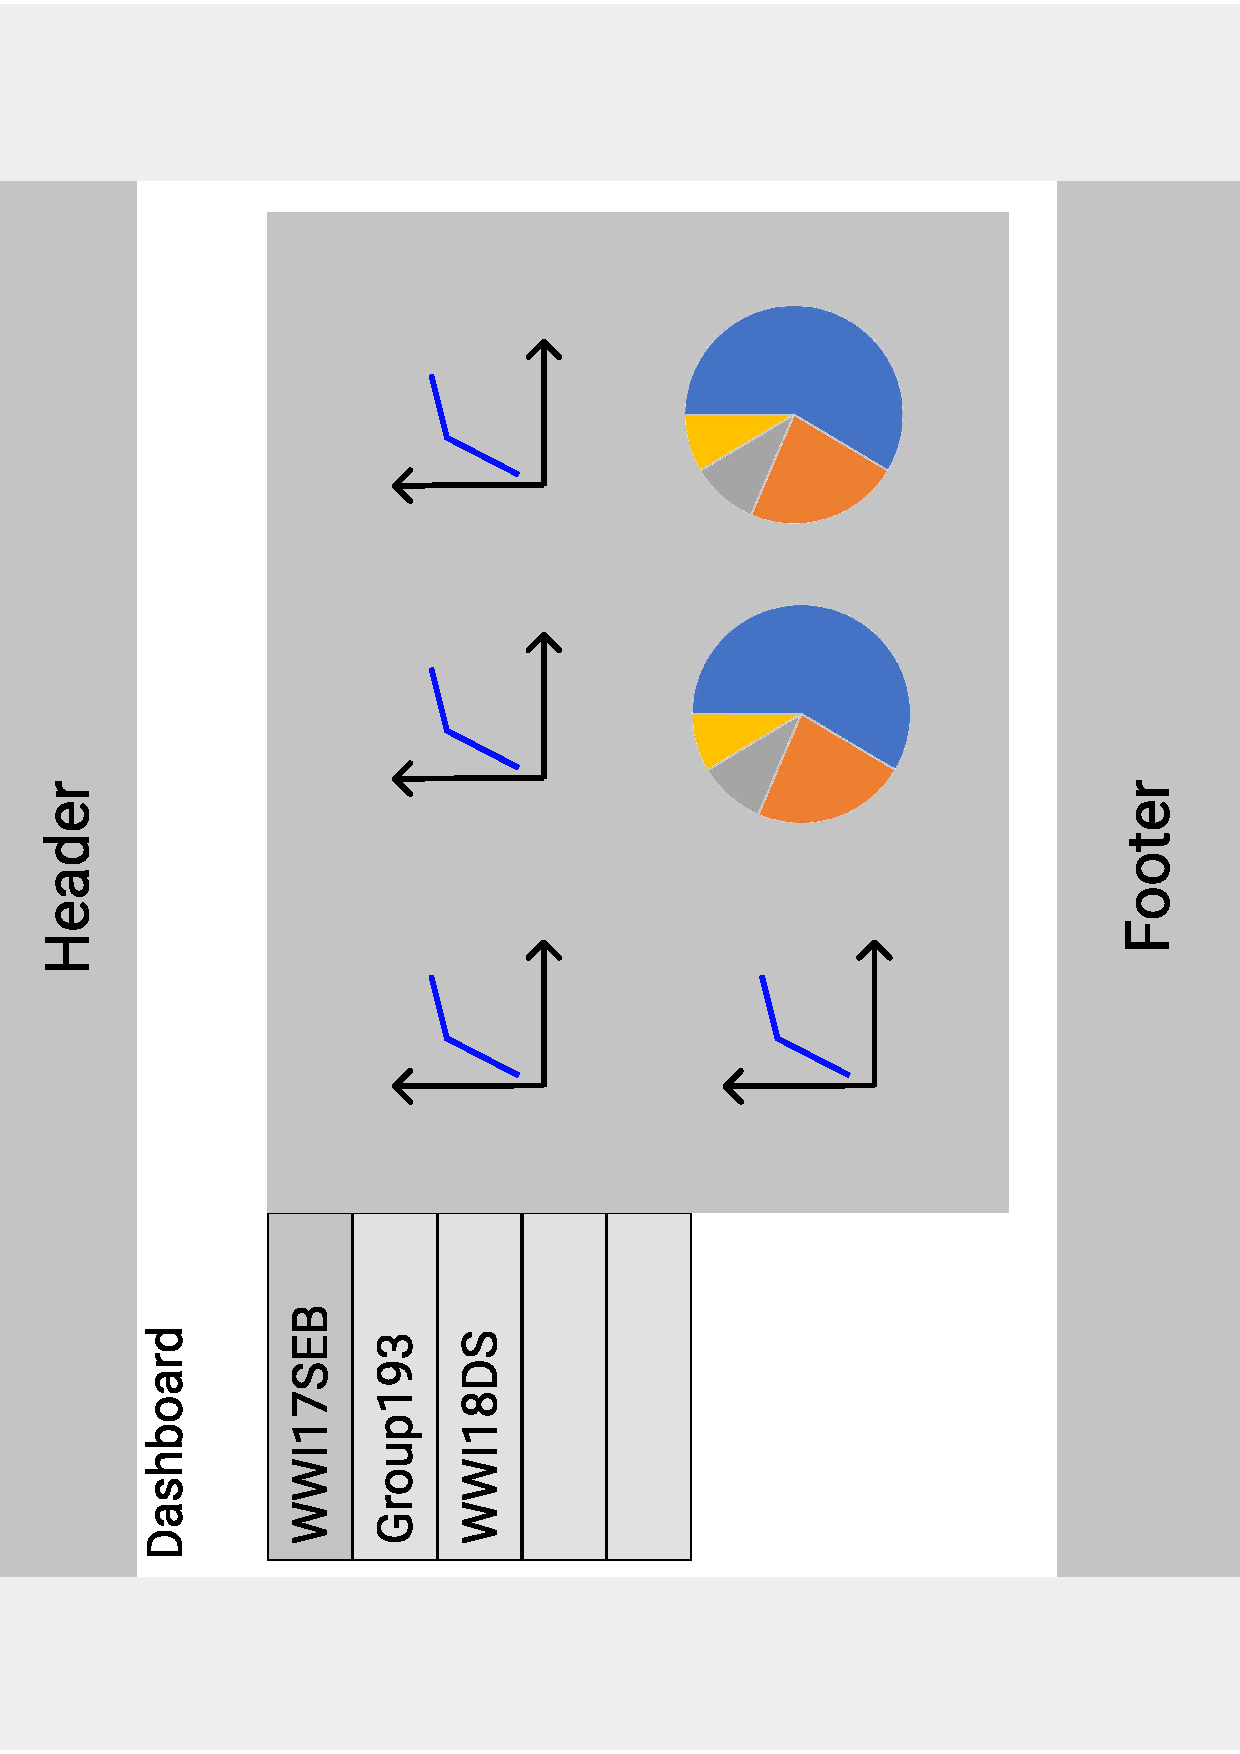
\includegraphics[width=0.7\textwidth]{img/konzeption/client/dashboard}
	\captionsetup{justification=centering, format=plain}
	\caption[Mock-Up des Dashboards]{Mock-Up des Dashboards \\\figma}
	\label{fig:MockDashboard}
\end{figure}



% !TeX root = ../../../master.tex

\subsection{Umfrage erstellen}
\label{ssec:UmfrageErstellen}

Das Herzstück der Applikation soll das Erstellen einer Umfrage sein.
Hier soll der Benutzer die Möglichkeit haben, eine Umfrage zu erstellen, die verschiedene Fragetypen beinhaltet.
Fragetypen sind exemplarisch:
%
\begin{itemize}
	\item Freitext (Single Input)
	\item Checkbox, Matrix (Multiple Choice)
	\item Radiogroup, Matrix (Single Choice)
	\item Dropdown
	\item Rating (Bewertungsskala)
	\item Boolean (Ja/Nein)
	\item Datepicker (Datumsfelder)
\end{itemize}
%

Die Abbildung~\myRefGeneral{fig:SurveyCreatorImplement} stellt den Umfrageeditor der Anwendung dar.
In diesem kann der Benutzer Umfragen erstellen und editieren.
Der Benutzer gibt der Umfrage einen Titel \engl{title} sowie eine Beschreibung \engl{description}.
Er kann mehrere Seiten anlegen und auch jeder Seite einen eigenen \emph{title} und eine eigene \emph{description} zuteilen. \newline
In der Toolbox (linke Seite) kann der Benutzer die verschiedenen Fragetypen über \emph{Drag \& Drop} auf die ausgewählte Seite schieben.
Hier kann der Benutzer die Frage und mögliche Auswahlmöglichkeiten (bei Single/Multiple Choice) definieren.

\begin{figure}[!htb]
	\centering
	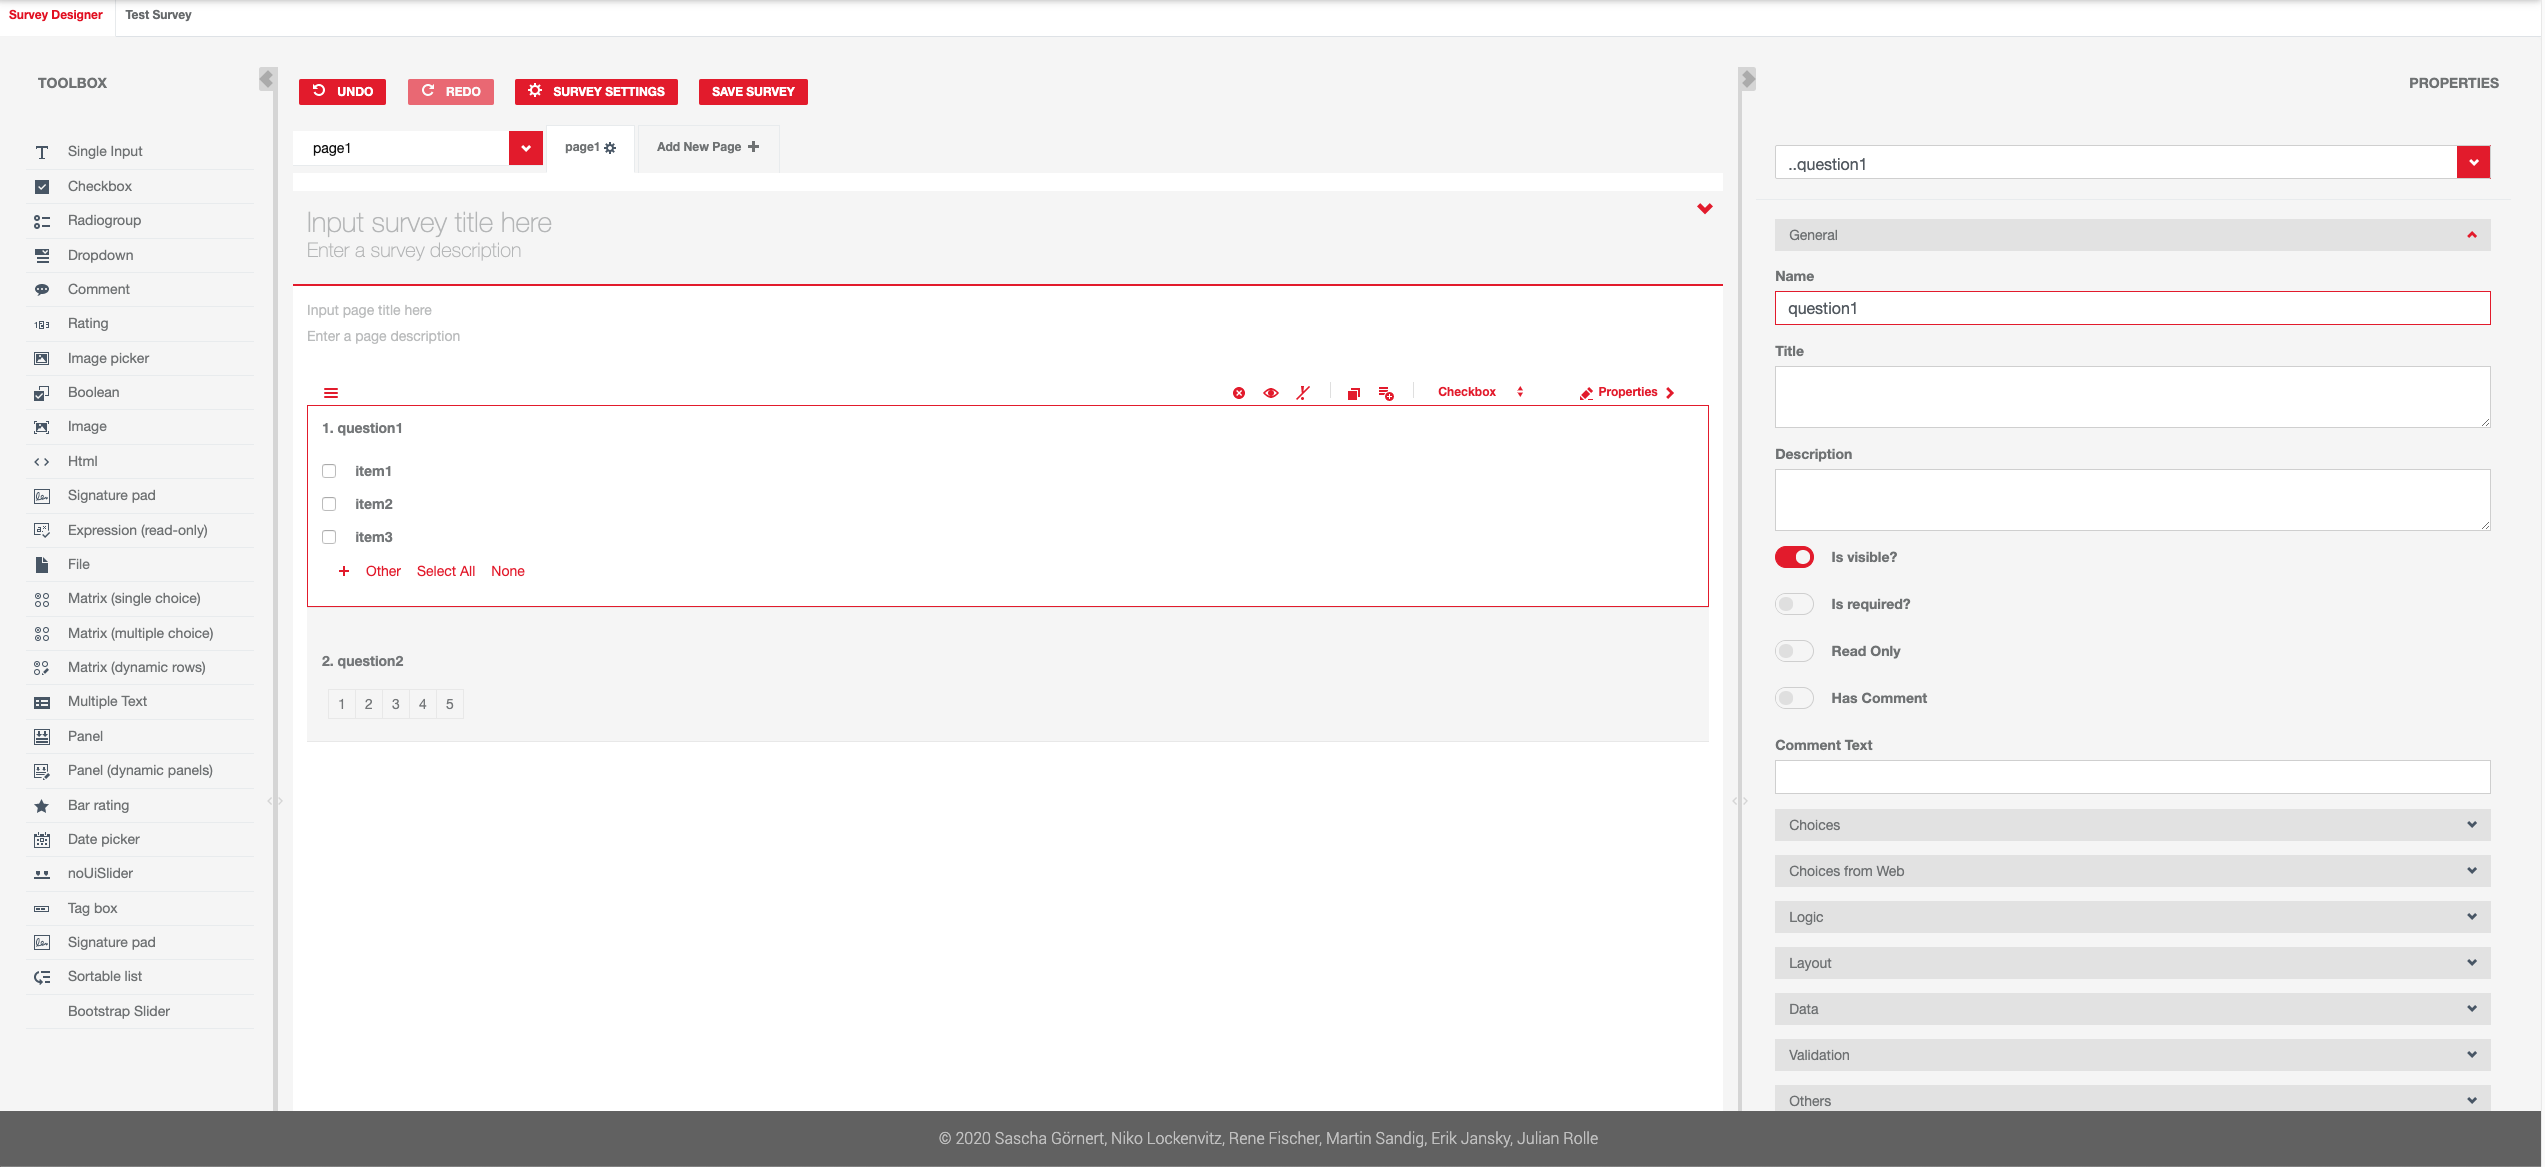
\includegraphics[width=0.95\textwidth, keepaspectratio]{img/client/CreateSurveyMaster.png}
	\captionsetup{justification=centering, format=plain}
	\caption[\acl{UI}: Erstellen einer Umfrage]{\acl{UI}: Erstellen einer Umfrage \\ \quelleScreenshot}
	\label{fig:SurveyCreatorImplement}
\end{figure}

Klickt der Benutzer auf die Schaltfläche \jinline|Test Survey|, werden die erstellten Umfragen dargestellt.
Dabei kann der Nutzer sehen, wie sich die Umfrage auf verschiedene Geräte, wie \zb einem iPhone 8, verhält.
Abbildung~\vref{fig:SurveyAnsicht} zeigt die Möglichkeit, die erstellte Umfrage auf einem bestimmten Gerät \engl{device} zu sehen (hier: Desktop).
Der Benutzer kann die Umfrage über eine Vorschau \engl{preview}, wie in Abbildung~\vref{fig:SurveyMobileAnsicht} dargestellt, auf verschiedenen mobilen Geräten betrachten.
Abbildung~\vref{fig:SurveyMobileAnsichtIPhone8} zeigt die erstellte Umfrage auf einem iPhone 8 an, wohingegen Abbildung~\vref{fig:SurveyMobileAnsichtAndroid} die Umfrage auf einem Android-Smartphone widerspiegelt.

\begin{figure}[!htb]
	\centering
	\captionsetup{justification=centering, format=plain}
	\subfigure[Ansicht der Umfrage]{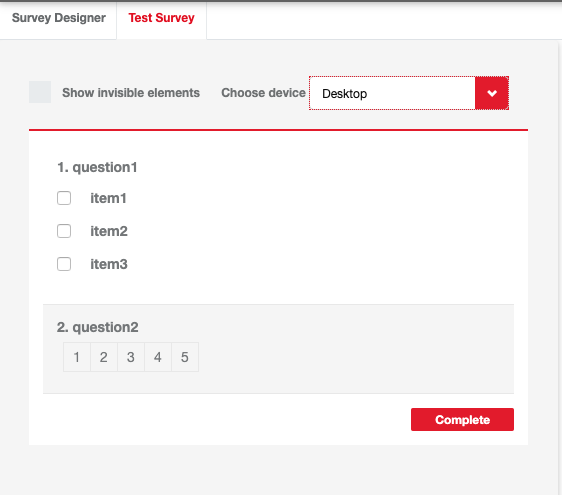
\includegraphics[width=0.48\textwidth]{img/client/CreateSurveyMaster_View1.png}\label{fig:SurveyAnsicht}}\hfill
	\subfigure[Auswahl verschiedener mobiler Ansichten]{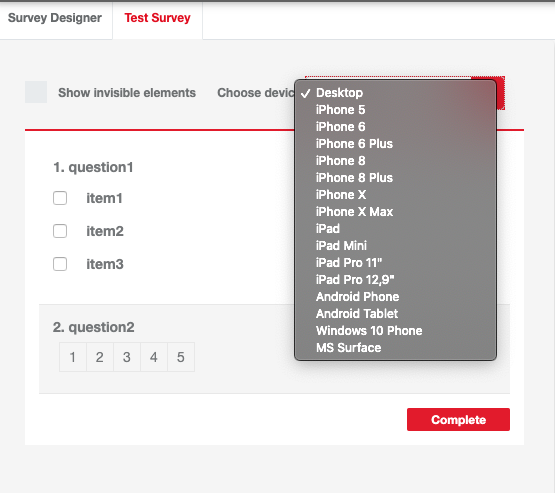
\includegraphics[width=0.48\textwidth]{img/client/CreateSurveyMaster_View2.png}\label{fig:SurveyMobileAnsicht}}\hfill
	\subfigure[Mobile Ansicht: iPhone 8]{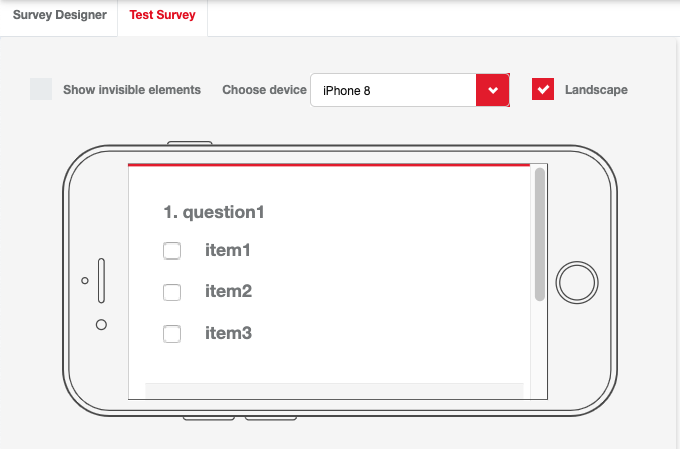
\includegraphics[width=0.48\textwidth]{img/client/CreateSurveyMaster_View3.png}\label{fig:SurveyMobileAnsichtIPhone8}}\hfill
	\subfigure[Mobile Ansicht: Android-Smartphone]{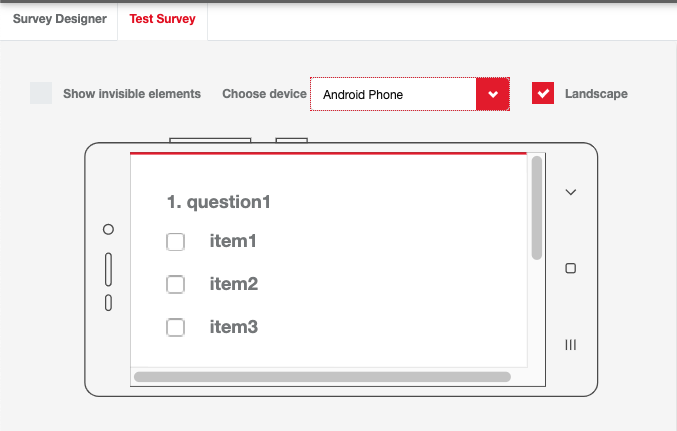
\includegraphics[width=0.48\textwidth]{img/client/CreateSurveyMaster_View4.png}\label{fig:SurveyMobileAnsichtAndroid}}
	\caption[\acl{UI}: Darstellung der erstellten Umfrage auf verschiedenen Geräten]{\label{fig:SurveyCreatorViewImplement}\acl{UI}: Darstellung der erstellten Umfrage auf verschiedenen Geräten \\ \quelleScreenshot}
\end{figure}

Über einen Knopf \jinline|Save Survey| kann der Benutzer die Umfrage speichern.
Zudem erhält der Nutzer ein visuelles Feedback über den Erfolg oder Nichterfolg des Erstellens der Umfrage.
Die erstellten Umfragen erscheinen im \emph{Survey Dashboard} (Kapitel~\vref{ssec:UmfrageDashboard}).


\subsection{Unterteilung der Gliederungsansichten}

\begin{itemize}
	\item Beschreibung der Mockups 
	 \begin{itemize}
		 \item Was haben wir uns bei den einzelnen Seiten gedacht -> mit den unterseiten erledigt
		 \item Wie sollten die Seiten grundsätzlich aussehen. (Brainstorming) -> im Grundgerüst
		 \item evtl. bissel auf Designthinking eingehen 
		 \item Welches tool haben wir dazu genutzt ->  FICK MA
	 \end{itemize}
	 \item Recherche zu vorhandenen Umfragetools --> (https://www.polly.ai/slack-poll, https://strawpoll.de/, https://www.limesurvey.org/de/, https://www.surveymonkey.de/, https://pingo.coactum.de/)
	 --> Ideensammlung und Marktrecherche
	 \item Grundlegende Idee der Einfachheit (evtl Gesamtkonzept)
	 \item Man könnte auf den User Journey eingehen
	 \item Anlehnung an DHBW farben sind vorgesehen
	 \item Orientierung an modernen Websites mit header und footer
	 \item Hinblick auf mobile usage
\end{itemize}

Das verwendete Tool zum Erstellen der Mockups ist Figma.
Figma\footnote{https://www.figma.com/} bietet eine Webanwendung an, in welcher einzelne Elemente per \emph{Drag&Drop} zu einer Arbeitsfläche hinzugefügt werden können. 
Die Auswahl der Elemente umfasst dabei Schrift, Formen und Farben, sowie weitere nützliche Eigenschaften, welche für den Anwendungsfall jedoch nicht relevant sind. 
Durch die große Auswahl an Strukturierungsmöglichkeiten, sind alle wichtigen Aspekte eines Mockup-Tools vorhanden.


\subsection{Bestimmung von Darstellungsformen}